\documentclass{article}
\usepackage{amsmath} % For mathematical symbols and environments
\usepackage{graphicx} % To include figures
\usepackage{geometry} % For adjusting margins
\usepackage{hyperref} % For clickable links (optional)

\geometry{a4paper, margin=1in} % Set page layout

\title{Image Restoration using ROF Model: Analysis Report}
\author{Dimtri Bolt} 
\date{\today} % today's date

\begin{document}
	
	\maketitle
	
	\section{Brief Explanation of Methods}
	
	\subsection{ROF Discretization and Difference Scheme}
	The Rudin-Osher-Fatemi (ROF) model aims to restore an image $u$ from a degraded observation $f$ by minimizing the functional:
	$$ \mathcal{F}(u) = \int \sqrt{\epsilon^{2} + |\nabla u|^{2}} \,dx\,dy + \frac{\lambda}{2} \int (u-f)^{2} \,dx\,dy $$
	where $\lambda$ is the fidelity parameter balancing data consistency and smoothing, and $\epsilon$ is a regularization parameter ensuring differentiability.
	
	The corresponding Euler-Lagrange PDE is:
	$$ \frac{u-f}{\lambda} - \nabla \cdot \left( \frac{\nabla u}{\sqrt{\epsilon^{2} + |\nabla u|^2}} \right) = 0 $$
	subject to Neumann boundary conditions ($\frac{\partial u}{\partial n} = 0$) on the image domain boundaries.
	
	This implementation solves the PDE using an iterative fixed-point method based on its discretized form. The discretization employs:
	\begin{itemize}
		\item \textbf{Finite Differences:} Standard central differences are used implicitly through forward/backward schemes.
		\begin{itemize}
			\item The gradient $\nabla u = (u_x, u_y)$ components are approximated using \textit{forward differences}:
			$$ (u_x)_{i,j} \approx u_{i,j+1} - u_{i,j} $$
			$$ (u_y)_{i,j} \approx u_{i+1,j} - u_{i,j} $$
			\item The divergence term $\nabla \cdot \mathbf{p}$ (where $\mathbf{p} = (p_x, p_y) = \frac{\nabla u}{\sqrt{\epsilon^2 + |\nabla u|^2}}$) is approximated using \textit{backward differences}:
			$$ (\nabla \cdot \mathbf{p})_{i,j} \approx (p_x)_{i,j} - (p_x)_{i,j-1} + (p_y)_{i,j} - (p_y)_{i-1,j} $$
		\end{itemize}
		\item \textbf{Neumann Boundary Conditions:} These are handled by using symmetric padding (`padarray(..., 'symmetric')`) before computing spatial differences near the boundaries. This effectively mirrors the image values across the boundary, enforcing a zero gradient perpendicular to the edge.
		\item \textbf{Iterative Solver:} The discretized PDE is rearranged into a fixed-point iteration scheme:
		$$ u^{(k+1)} = f - \lambda \cdot \nabla \cdot \left( \frac{\nabla u^{(k)}}{\sqrt{\epsilon^2 + |\nabla u^{(k)}|^2}} \right) $$
		where $u^{(k)}$ is the solution at iteration $k$. The iteration starts with $u^{(0)} = f$ and continues until the relative change between successive iterations ($||u^{(k+1)} - u^{(k)}|| / ||u^{(k)}||$) falls below a specified tolerance (\texttt{tol = 1e-4}) or a maximum number of iterations (\texttt{max\_iter = 100}) is reached.
	\end{itemize}
	This scheme is implemented in the MATLAB function \texttt{smooth\_image\_rof.m}.
	
	\section{Interpretation of Results}
	
	\subsection{MSD Plot Analysis}
	The plot 'Stacked MSD Surfaces for R, G1, G2, B Planes' (shown in Figure \ref{fig:msd_plot}) displays the Mean Square Difference (MSD) between the original noisy color plane ($f$) and the ROF-smoothed version ($u$) as a function of the parameters $\lambda$ and $\epsilon$. The MSD is calculated as:
	$$ \text{MSD}(f,\lambda,\epsilon) = \sqrt{\frac{\sum_{i,j}(u_{i,j} - f_{i,j})^{2}}{H \cdot W}} $$
	Each colored surface represents one of the four color planes (Red, Green1, Green2, Blue) extracted from the Bayer mosaic. The surfaces are stacked vertically with transparency to allow comparison.
	
	\begin{figure}[h!]
		\centering
		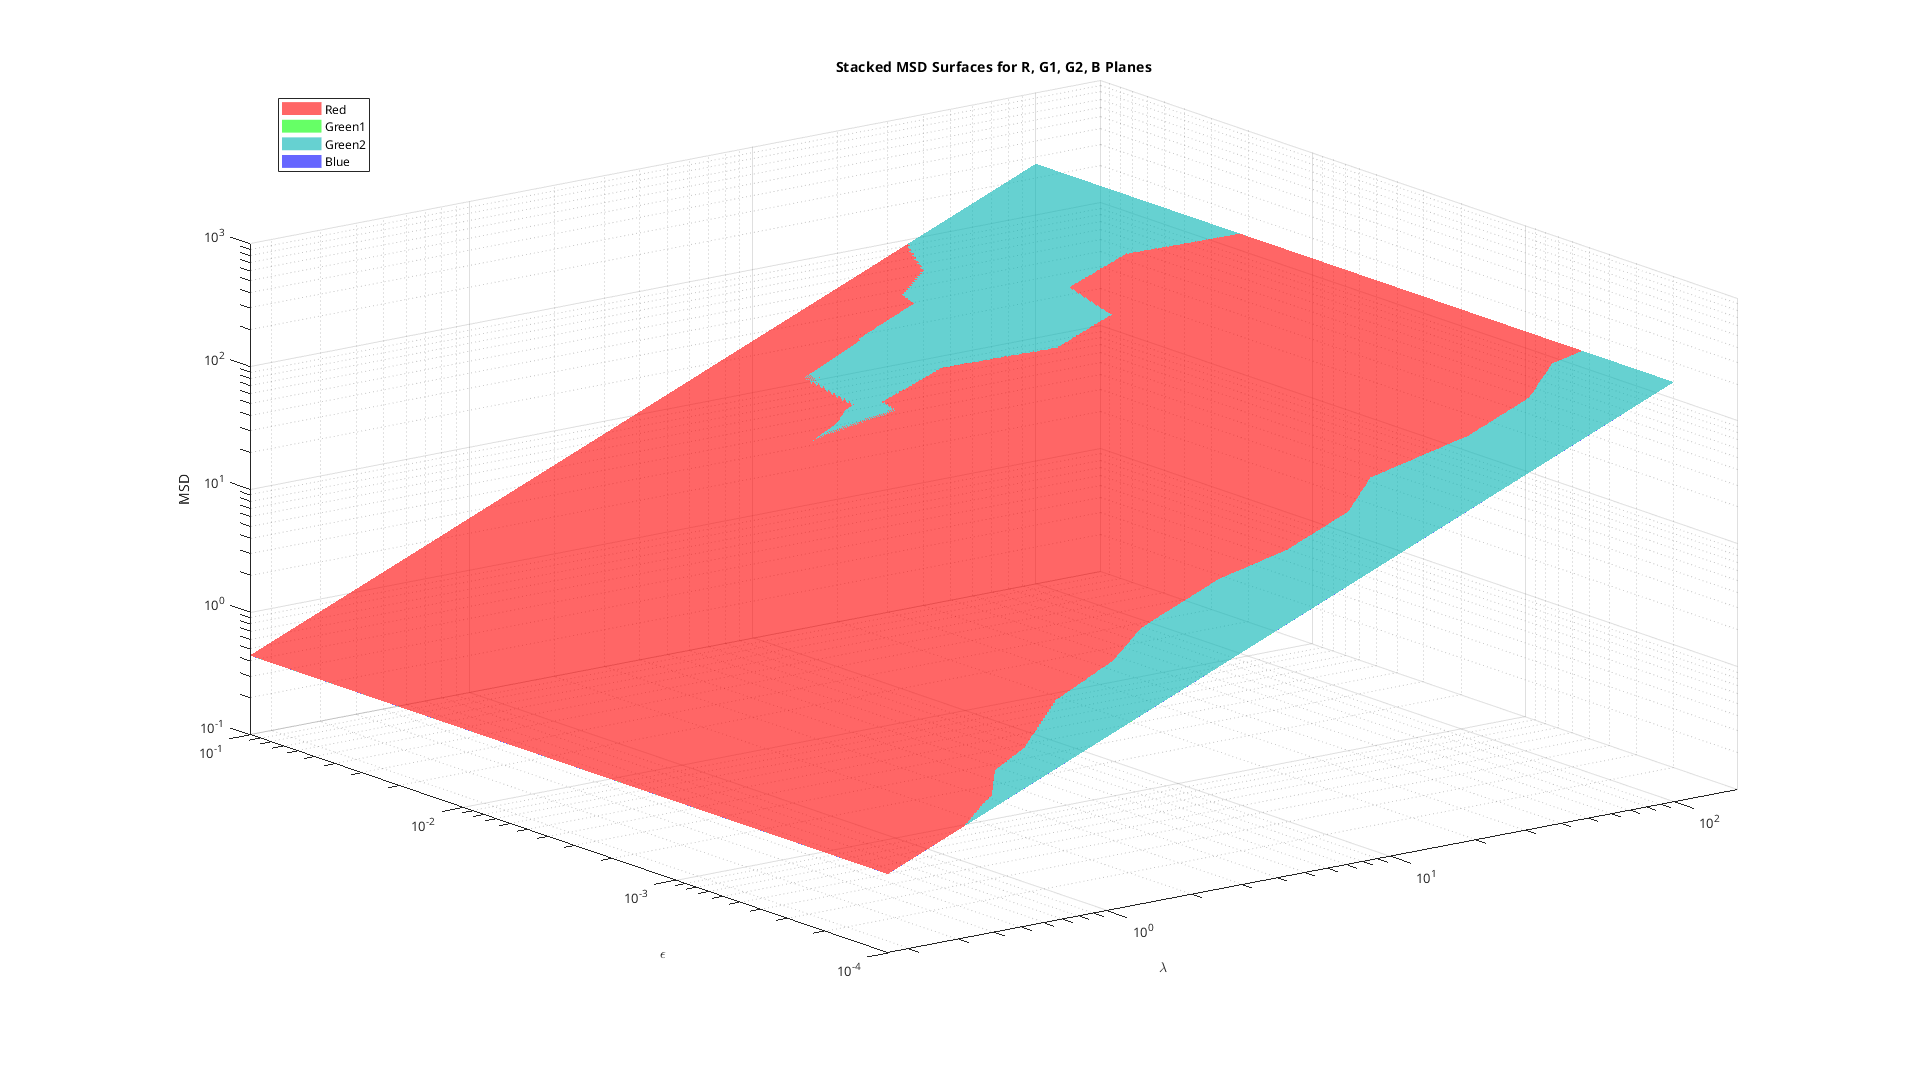
\includegraphics[width=0.8\textwidth]{/home/dimitri/Documents/Algorithms/Spring/ImageRestoration/msd_plot.png}
		\caption{Stacked MSD Surfaces vs. $\lambda$ and $\epsilon$ for R, G1, G2, B planes.}
		\label{fig:msd_plot}
	\end{figure}
	
	\textbf{Dependence on $\lambda$:}
	The parameter $\lambda$ controls the weight of the data fidelity term $\frac{1}{2} \int (u-f)^2$.
	\begin{itemize}
		\item For \textit{small} $\lambda$, the gradient term $\int \sqrt{\epsilon^2 + |\nabla u|^2}$ dominates. The model prioritizes smoothness, potentially oversmoothing the image ($u$ becomes very different from $f$), leading to a \textit{higher} MSD.
		\item For \textit{large} $\lambda$, the fidelity term dominates. The model forces the solution $u$ to be very close to the noisy input $f$. This results in less smoothing and a \textit{lower} MSD, as the difference $u-f$ approaches zero.
	\end{itemize}
	Therefore, the MSD is expected to decrease as $\lambda$ increases. The plot likely shows this trend, though calling it strictly "linear" might be an oversimplification; the relationship is generally monotonic decreasing but non-linear, especially when viewed on logarithmic scales. The rate of decrease diminishes as $u$ gets very close to $f$.
	
	\textbf{Dependence on $\epsilon$:}
	The parameter $\epsilon$ regularizes the gradient term, essentially setting a threshold below which gradient magnitudes do not heavily influence the cost.
	\begin{itemize}
		\item For \textit{very small} $\epsilon$, the term $\sqrt{\epsilon^2 + |\nabla u|^2} \approx |\nabla u|$ (Total Variation). The model strongly penalizes any gradients, leading to significant smoothing and potentially piecewise constant results. This strong smoothing might increase the MSD if it removes actual image features along with noise.
		\item For \textit{large} $\epsilon$, the term $\sqrt{\epsilon^2 + |\nabla u|^2} \approx \epsilon + \frac{|\nabla u|^2}{2\epsilon} + \dots$. The gradient's influence is down-weighted relative to the constant $\epsilon$. The model allows steeper gradients with less penalty, resulting in less smoothing. As $\epsilon$ becomes very large, the first term's contribution to the functional becomes less dependent on $\nabla u$, and the fidelity term (scaled by $\lambda$) dictates the solution more, potentially making $u$ closer to $f$.
	\end{itemize}
	The observation that there appears to be "no dependence on $\epsilon$" in the plot might be due to several factors:
	\begin{enumerate}
		\item The chosen range for $\epsilon$ might be too high, placing the analysis in a regime where MSD is less sensitive to $\epsilon$.
		\item The variation in MSD due to $\epsilon$ might be much smaller than the variation due to $\lambda$, making it less apparent on the combined plot, especially with logarithmic axes potentially compressing the visual effect.
		\item There might be an interaction effect, where the influence of $\epsilon$ is only significant for certain ranges of $\lambda$.
	\end{enumerate}
	Fundamentally, MSD \textit{should} depend on $\epsilon$, as $\epsilon$ directly influences the degree of smoothing applied, which in turn affects the difference $u-f$. A lack of apparent dependence warrants closer inspection of the parameter ranges and plot scales.
	
	\section{Discussion of Noise Differences Between Color Planes}
	
	\subsection{Measuring Noise using ROF}
	In this context, the "noise" is interpreted as the high-frequency variations present in the observed image $f$ that are removed by the ROF smoothing process to produce the restored image $u$. The ROF model, particularly for appropriate $\lambda$ and $\epsilon$, aims to separate the underlying structure ($u$) from the noise ($n \approx f-u$).
	The Mean Square Difference (MSD) serves as a quantitative measure of the "amount" of information removed during smoothing. By finding the parameters $(\lambda_{opt}, \epsilon_{opt})$ that minimize the MSD for a given plane, we find the ROF solution $u_{opt}$ that is closest (in the mean square sense) to the original $f$. While not a direct measure of noise power in the traditional signal processing sense, the minimum MSD achieved provides a relative measure of the noise level removed by ROF across the different color planes. A lower minimum MSD suggests either less noise was present initially, or the noise structure was more amenable to removal by ROF smoothing.
	
	\subsection{Analysis of Noise Statistics (via MSD)}
	By examining the stacked surfaces in Figure \ref{fig:msd_plot}, we can compare the MSD values across the R, G1, G2, and B planes.
	\begin{itemize}
		\item \textbf{Relative Noise Levels:} The plane whose surface sits consistently lower than the others, especially in the region of minimum MSD values, can be inferred to be the "least noisy" as interpreted by the ROF model. Conversely, the plane with the highest surface suggests it contains more noise (or features interpreted as noise by ROF). Based on typical sensor characteristics and the Bayer pattern, one might expect the Green channels (G1, G2) to potentially exhibit lower noise or different noise characteristics compared to Red and Blue, as there are twice as many green sensors, often contributing more to luminance detail. Visual inspection of the plot is required to confirm which planes yield lower minimum MSD values.
		\item \textbf{Bayer Pattern Speculation (Two Green Planes):} Digital camera sensors use a Color Filter Array (CFA), most commonly the Bayer pattern (RGGB), to capture color information with a single sensor layer. The human visual system is more sensitive to green light, which carries most luminance information. Having twice as many green pixels (G1, G2) as red or blue allows the camera to capture finer luminance detail and potentially reduce luminance noise through averaging during the demosaicing process (which reconstructs the full-color image). While G1 and G2 pixels capture the same color, their surrounding neighbors in the RGGB grid are different, which can lead to slight variations in their values after processing or potential differences in noise characteristics depending on sensor readout patterns or demosaicing algorithms, although ideally they should represent similar noise levels from the same (green) spectral band. Comparing the MSD surfaces for G1 and G2 can reveal if they exhibit significantly different noise levels in the raw data.
	\end{itemize}
	
	\section{Software Structure}
	
	\subsection{Software Components}
	The image restoration software consists of the following MATLAB script files:
	\begin{itemize}
		\item \texttt{basic\_script.m}: Performs initial setup. Reads the raw image file (e.g., \texttt{DSC00099.ARW}), extracts metadata, and separates the Bayer mosaic data into four distinct color planes (R, G1, G2, B) stored in the variable \texttt{Iplanar}. It also includes visualization steps.
		\item \texttt{smooth\_image\_rof.m}: Implements the core ROF algorithm. Takes a single image plane ($f$) and parameters ($\lambda, \epsilon$) as input and returns the smoothed image ($u$). Handles scalar or vector parameters, Neumann boundary conditions, GPU acceleration (if available), and parallel CPU processing (using \texttt{parfor} for vector parameters if no GPU).
		\item \texttt{calculate\_msd.m}: Computes the Mean Square Difference (MSD) between an input image plane ($f$) and its ROF-smoothed version. It calls \texttt{smooth\_image\_rof} internally to get the smoothed image $u$ for the given parameters ($\lambda, \epsilon$) before calculating the MSD.
		\item \texttt{run\_rof\_analysis.m}: The main driver script that orchestrates the entire analysis. It calls \texttt{basic\_script.m}, defines parameter ranges, manages the processing of each color plane (including chunking for GPU memory management), calls \texttt{calculate\_msd} for parameter sweeps, collects results, and generates the final stacked MSD surface plot.
	\end{itemize}
	
	\subsection{How to Launch the Software}
	To run the analysis:
	\begin{enumerate}
		\item Ensure all MATLAB script files (\texttt{run\_rof\_analysis.m}, \texttt{basic\_script.m}, \texttt{smooth\_image\_rof.m}, \texttt{calculate\_msd.m}) are in the MATLAB path or the current working directory.
		\item Ensure the raw image file (\texttt{DSC00099.ARW}) is located in the path expected by \texttt{basic\_script.m} (e.g., in a subdirectory named \texttt{images}).
		\item Open MATLAB.
		\item Run the main driver script by typing its name in the Command Window or by opening it in the Editor and pressing the 'Run' button:
		\begin{verbatim}
			>> run_rof_analysis
		\end{verbatim}
	\end{enumerate}
	The script will then execute the full analysis and produce the MSD plot. Progress messages will be displayed in the Command Window.
	
	\subsection{Software Logic Flow}
	The execution proceeds as follows:
	\begin{enumerate}
		\item \texttt{run\_rof\_analysis.m} is executed.
		\item It first calls \texttt{basic\_script.m} to load the raw image data and extract the four color planes (R, G1, G2, B) into the variable \texttt{Iplanar}.
		\item It defines the vectors of parameters \texttt{lambda\_vec} and \texttt{epsilon\_vec} over which the analysis will be performed.
		\item It sets up parameters for processing the parameter grid in chunks to manage GPU memory (\texttt{combinations\_per\_chunk}, \texttt{num\_chunks}).
		\item It initializes a cell array (\texttt{msd\_results}) to store the final MSD matrices for each plane.
		\item It enters a loop iterating through the four color planes (j=1 to 4):
		\begin{itemize}
			\item Extracts the current plane from \texttt{Iplanar} and converts it to \texttt{single} precision.
			\item Enters a second loop iterating through the defined chunks:
			\begin{itemize}
				\item Determines the subset of (\texttt{lambda}, \texttt{epsilon}) pairs for the current chunk.
				\item Calls \texttt{calculate\_msd} with the current plane and the parameter subset for this chunk.
				\item Inside \texttt{calculate\_msd}:
				\begin{itemize}
					\item It calls \texttt{smooth\_image\_rof} with the same inputs.
					\item \texttt{smooth\_image\_rof} performs the iterative ROF smoothing. If a GPU is available and parameters are vectors, it uses an internal batched GPU computation; otherwise, it uses \texttt{parfor} on the CPU for vector parameters.
					\item \texttt{smooth\_image\_rof} returns the smoothed image(s) $u$.
				\end{itemize}
				\item \texttt{calculate\_msd} computes the MSD between $f$ and $u$ for the chunk and returns the result (\texttt{msd\_chunk}).
			\end{itemize}
			\item The main script (\texttt{run\_rof\_analysis.m}) carefully maps the results from \texttt{msd\_chunk} back into the correct positions in the overall \texttt{msd\_results\{j\}} matrix for the current plane.
			\item (Optionally, GPU memory is reset between chunks).
		\end{itemize}
		\item After processing all chunks for all four planes, \texttt{run\_rof\_analysis.m} uses the completed \texttt{msd\_results} matrices and \texttt{meshgrid}/\texttt{surf} to generate the final stacked 3D surface plot showing MSD vs. $\lambda$ and $\epsilon$ for all planes.
	\end{enumerate}
	
	\section{GPU Memory Considerations}
	
	\subsection{GPU Memory Issues Encountered}
	During the execution of the analysis with vector inputs for $\lambda$ and $\epsilon$ on a machine equipped with a GPU, an "Out of memory on device" error was encountered. This occurred specifically within the \texttt{smooth\_image\_rof.m} function when processing multiple parameter combinations simultaneously using the GPU-accelerated code path.
	
	The root cause lies in the strategy employed for GPU vectorization within \texttt{smooth\_image\_rof}. To process $K \times L$ parameter combinations efficiently, the input image $f$ is replicated $K \times L$ times into a large 4D \texttt{gpuArray} (\texttt{f\_big}). The subsequent fixed-point iteration requires numerous intermediate 4D arrays of the same large size (\texttt{[H, W, K, L]}) to be stored concurrently in GPU memory (e.g., \texttt{uk}, \texttt{up}, \texttt{ux}, \texttt{uy}, \texttt{mag}, \texttt{px}, \texttt{py}, \texttt{div\_p}, \texttt{unew}). For the image size ($H \approx 2000, W \approx 3000$) and the chosen parameter grid size ($K=15, L=10$, total $150$ combinations), the cumulative size of these temporary arrays significantly exceeded the available GPU RAM (e.g., 8.5 GB), leading to the memory allocation failure (specifically noted during a \texttt{padarray} call).
	
	\subsection{Resolution of GPU Memory Issues}
	The out-of-memory issue is resolved by implementing a \textbf{chunking} strategy within the main driver script, \texttt{run\_rof\_analysis.m}, rather than attempting to process the entire $K \times L$ parameter grid in a single call on the GPU.
	
	The key variables controlling this strategy are:
	\begin{itemize}
		\item \texttt{num\_total\_combinations}: Calculated simply as $K \times L$, the total number of $(\lambda, \epsilon)$ pairs in the full grid.
		\item \texttt{combinations\_per\_chunk}: A user-defined parameter specifying the maximum number of parameter combinations to process in a single call to \texttt{calculate\_msd} (and thus \texttt{smooth\_image\_rof}). This value is chosen small enough such that the peak memory usage for processing this many combinations stays within the available GPU RAM. A value of 15 was used as a starting point.
		\item \texttt{num\_chunks}: Calculated as $\lceil \texttt{num\_total\_combinations} / \texttt{combinations\_per\_chunk} \rceil$. This determines the number of iterations required in the chunking loop to cover the entire parameter grid.
	\end{itemize}
	The \texttt{run\_rof\_analysis.m} script now includes an outer loop iterating \texttt{num\_chunks} times. In each iteration, it identifies a small subset of (\texttt{lambda}, \texttt{epsilon}) pairs corresponding to the current chunk. It then calls \texttt{calculate\_msd} with only these limited parameter vectors. Consequently, the internal GPU processing within \texttt{smooth\_image\_rof} only needs to handle a much smaller batch size (at most \texttt{combinations\_per\_chunk}), drastically reducing the peak GPU memory requirement for temporary arrays. The results from each chunk are then collected and carefully reassembled into the final full MSD matrix for each color plane. This approach effectively trades potentially longer overall execution time (due to multiple function calls and potentially less optimal GPU utilization per call) for the ability to complete the computation within the constrained GPU memory environment.
	
\end{document}